\chapter{Data}\label{CH_01}

SED fitting is now a standard technique of deriving stellar mass for a large set of galaxies. In this method multi-band photometry for a given galaxy is fitted to a series of a templates predicted by a certain population synthesis model. The best-fit template gives the parameters of the galaxy, including its redshift and mass.
Historically, population synthesis models were using restframe optical photometry. One caveat is the degeneracy between the dust extinction and age of the stellar population, as both make the color of galaxy red, i.e. galaxy can be red because it is intrinsically red with no young massive star and ongoing star-formation, or it can be very dusty, or it could be metal-rich and metals effectively absorb light in the bluer bands. Solution to this is to implement restframe near-IR where light suffers much less extinction (comparing to restframe UV and optical) and thus the degeneracy can be broken.
We aim to build the largest sample of galaxies with optical and near-IR photometry over a large sky area. The natural choice for us then is to use optical Sloan Digital Sky Survey (SDSS) and IR all-sky data from Wide-Field Infrared Survey Explorer (WISE).

\section{SDSS}
SDSS \citep{York2000} was an imaging and spectroscopic survey with a dedicated 2.5m telescope at Apache Point Observatory, New Mexico, USA. Imaging is performed by 142 mega-pixel camera as shown on Figure~\ref{fig:sdss}, that uses the drift-scan mode in five broad optical filters, namely \textit{ugriz} \citep{1998AJ....116.3040G} spanning from 3,000 to 10,000 {\AA}. While the spectroscopic survey is still carried on, the imaging survey has been completed and by now it covers 14,555 $deg^{2}$ of unique sky area with pixel scale 0.396". Exposure time is 53.9 seconds per band. An SDSS run consists of six parallel scanlines. The skylines are 13.5' wide with the gaps between them of relatively same size. Two interleaving runs make stripe that consists of total 12 scanlines (columns).

\begin{figure}[!ht]
\centerline{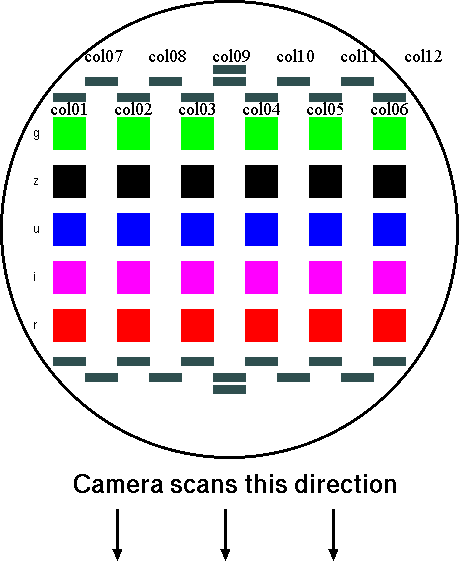
\includegraphics[width=4in]{Figures/sdss_camera.png}}
\caption{The camera used for imaging. It consists of 30 photometric CCDs, that are arranged in 6 columns of 5 each. Camera is drifted in the way that each column has permanent Declination during the run and all 5 filters in a column consequently go over the same field}
\label{fig:sdss}
\end{figure}

\subsection{Stripe 82}
Single-pass images are shallow (magnitude limit in r-band is 22.2 AB) and is not suitable for our purposes. For that reason we shall use Stripe 82, a $\approx300$ sq.degree area on the Celestial Equator in the South Galactic Cap in the Fall \citep{Adelman-McCarthy2007}. Stripe 82 is a deep survey stripe that spans $20h < RA < 4h$ and $-1.26 < Dec < 1.26$. This area was repeatedly used for calibration purposes and was scanned 70-90 times depending on RA. The advantage of these multiepoch images was quickly anticipated by various teams who stacked it and created co-added images. Annis et al. \citep{Annis2014} produced the first version of stacked images. They combined images available by December, 2005 (20-35 runs) and achieved magnitude limit 1-2 mag deeper then single-epoch SDSS products. results were published in SDSS Data Release 7 (DR7). Several teams produced their own co-adds using different strategy for the selection and post-processing of images (e.g. Huff et al.2014 \citep{2014MNRAS.440.1296H}, Jiang et al. 2009 \citep{2009AJ....138..305J}). It is important to outline that images were taken under different photometric conditions (e.g. significant moonlight and poor seeing in several runs performed in 2005-2007) and thus certain selection of the images has to be performed.

Jiang et al. 2014 (J14) \citep{Jiang2014} released a new version of co-adds in which only images that had been taken under perfect photometric conditions were used. These co-adds, that we shall use in our work are in general 0.2 mag deeper than in Annis et al. and 2 mag deeper than single-epoch SDSS images (see fig 7 in J14) and reach $5\sigma$ detection limit of 23.9, 25.1, 24.6, 24.1, and 22.8 AB magnitudes in bands u-, g-, r-, i- and z- respectively. 

\subsection{Structure of SDSS Stripe 82 files}

	We use description from J14 to present the structure of optical data. An SDSS run (strip) consists of six parallel scanlines, identified by camera columns (Figure~\ref{fig:sdss}). The scanlines are 13.5 arcmin wide, with gaps of roughly the same width, so two interleaving strips make a stripe. That creates the following sequence of columns in the direction of increasing declination:
$col01 \rightarrow col07 \rightarrow col02 \rightarrow col08 \rightarrow col03 \rightarrow col09 \rightarrow col04 \rightarrow col10 \rightarrow col05 \rightarrow col11 \rightarrow col06 \rightarrow col12$.

%\begin{figure}[!ht]
%\includegraphics[width=6in]{THE ONE THAT HAOJING SENT ME}
%\caption{sample text}
%\label{fig:sdss_s82}
%\end{figure}

The size of each SDSS image is 1489 x 2048 pixels, or roughly 9.8' x 13.5' (RA x Dec), with a pixel size of 0.396" and an average full width at half maximum (FWHM) of $\sim1.5"$ in u-band, $\sim1.3"$ in g-band, and $\sim1"$ in r-, i-, and z-bands. In total there are 401 SDSS images in each column and overall $12 \cdot 401 \cdot 5 = 24,060$ SDSS images. Between any two adjacent images there is an overlap region with a width of 128 pixels along the scan direction. Catalogs that we produce will have duplicate sources for such regions and it shall be removed in the post-processing stage by internal matching of all sources in the final catalog using the matching radius of 1.2". This radius was determined empirically to be the largest at which we do not have false rejections - rejection of two sources that lay very close to each other on the line of sight.\\ 
Images are named by their band, column and sequential number, e.g. $S82\_11x\_222.fits$, where 11 is the column number, x - letter for one of the five bands, and 222 - sequential number. Each SDSS image has a corresponding weight.fits image, that records relative weights at individual pixels.

\section{WISE}

WISE \citep{Wright2010} is a near-IR space observatory that was launched in December 2009 and mapped the entire sky with sensitivity far better than that of its predecessors, IRAS \citep{Neugebauer1984} and DIRBE \citep{Silverberg1993}. With a 0.4 m telescope on board always pointing at 90 degrees solar elongation, WISE made successful scans of the entire sky in four bands, namely w1 ($3.4 \mu m$), w2 ($4.6 \mu m$), w3 ($12 \mu m$) and w4 ($22 \mu m$). Its observations have very wide range of applications from search of near-Earth asteroids and brown dwarfs to the studies of the most luminous galaxies in the Universe.

\subsection{unWISE}

WISE data are published as a set of co-added data. Stacks were created by the WISE/NEOWISE team using the first 13 months of data (AllWISE release) and are available at NASA/IPAC \fnurl{Infrared Science Archive}{http://irsa.ipac.caltech.edu}. Original images were intentionally blurred by the WISE point spread function (PSF) for better detection of deep single sources. But that leads to the blending problem in the crowded fields and also decreases the signal-to-noise ratio (SNR) due to the broadening of the PSF. D.Lang \citep{Lang2014e} (D14) has produced custom “unWISE” stacks analogous to the AllWISE images, but at the full spatial resolution of the instrument - 2.75"/pixel. Example of the WISE team stacks and deconvolved unWISE stacks can be seen at Figure 2 in D14. unWISE images are appropriate for photometry in the crowded fields and they preserve the available signal-to-noise and we shall use it with SDSS Stripe 82 data in this project.

\subsection{Structure of unWISE files}

Structure and naming convention of unWISE files is taken from \fnurl{unwise.me}{http://unwise.me/data}. The unWISE coadds are on the same tile centers as the WISE images: 18,240 tiles per band, 1.56 x 1.56 degrees each. The tiles are named by their RA, Dec center: tile "0591p530" is at RA = 59.1, Dec = +53.0 degrees; i.e., the first four digits of the tile name is $int(RA \cdot 10)$, then "p" for +Dec and "m" for -Dec, then three digits of $int(abs(Dec)\cdot 10)$. For each tile and band w1-w4, several images are produced, we shall list only the ones that we make use of:

-- unwise-0000p000-w1-img-m.fits - "Masked" image, 2048 x 2048 pixels, TAN projected at 2.75"/pixel. Background-subtracted, in units of "Vega nanomaggies" per pixel: $mag = -2.5 \cdot (log_{10}(flux) - 9)$. This is our science image. The word "masked" means that some pixels will have no unmasked pixels and no measurement at all: pixel value 0 and infinite uncertainty.

-- unwise-0000p000-w1-std-m.fits - Sample standard deviation (scatter) of the individual-exposure pixels  contributing to this coadd pixel. This will be large if, for example, the source is variable.\\

One unWISE FITS image may cover up to 72 SDSS images within its footprint. We shall call one unWISE image or a set of SDSS images within this area "a frame".

For each coordinate in RA there are 3 unWISE images that covers all 12 SDSS columns (ranging from -1.26 < Dec < +1.26). We call such a set of three unWISE images a frame. One frame fits up to 72 SDSS images. Two adjacent frames overlap by $\sim2.9'$ and sources that appear in such regions will be duplicated. Such sources, as in the case of the overlapping SDSS images, shall be removed in the post-processing stage.


